\documentclass{beamer}
\usepackage{graphicx}
\usetheme{CambridgeUS}
\usecolortheme{seahorse}

\mode<presentation>

\title{Optimizing paths for autonomous flying robots \\ using reinforcement learning}
\author[Martijn van der Veen]{Martijn van der Veen}
\date[05-04-2011]{5 april 2011}

\begin{document}

\begin{frame}
  \titlepage
\end{frame}

\section*{Outline}

\begin{frame}
  \tableofcontents
\end{frame}


\section{Goal}

\begin{frame}
  \frametitle{Goal}
  \begin{block}{Goal}
    Optimizing paths for an vision-based autonomous flying robot using reinforcement learning \\

    Preferably as general as possible
  \end{block}
\end{frame}

\section{Reinforcement Learning}
\begin{frame}
  \frametitle{Reinforcement learning}
  \begin{figure}
    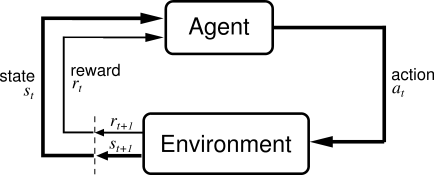
\includegraphics[width=0.8\textwidth]{img/RL}
    \caption{Reinforcement Learning}
  \end{figure}
  Mainly used in simple simulated problems (i.e. games)
  %\begin{itemize}
  %  \item 
  %\end{itemize}
\end{frame}


% TODO: hier uitleggen hoe aan te pakken
% zoeken naar:  learning parameters "reinforcement learning"
\section{Possible approaches}
\begin{frame}
  \frametitle{Possible approaches}
  \begin{itemize}
    \item Path planning in whole environment
    \begin{itemize}
      \item Extract features from images $\rightarrow$ State
      \item A priori path
      \item Learn optimal path in state-space
    \end{itemize}
    \item Estimating parameters for pre-defined path
    \begin{itemize}
      \item Reinforcement Parameter Control
      \item Learn optimal parameters
    \end{itemize}
    %\begin{itemize}
    %  \item Angle of cross
    %  \item Distance from pylon
    %  \item Speed
    %\end{itemize}
  \end{itemize}
\end{frame}



\section{Practical Problem}

\begin{frame}
  \frametitle{Practical problem}
  \begin{figure}
    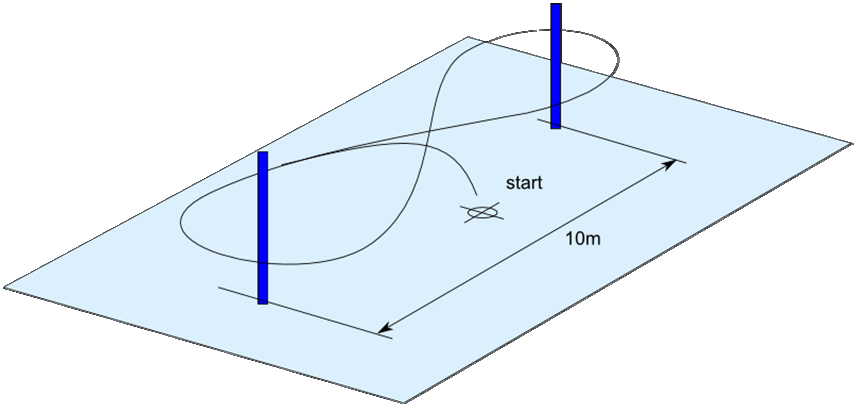
\includegraphics[width=0.8\textwidth]{img/8}
  \end{figure}
  \begin{itemize}
    \item International Micro Air Vehicle (IMAV) Flight Competition
    \item Pylon Challenge: fly in figure 8's around poles
    \item Learn optimal path
    %\begin{itemize}
    %  \item Angle of cross
    %  \item Distance from pylon
    %  \item Speed
    %\end{itemize}
  \end{itemize}
\end{frame}

\section{Tools}

\subsection{AR.Drone}
\begin{frame}
  \frametitle{Tool: AR.Drone}
  \begin{figure}
    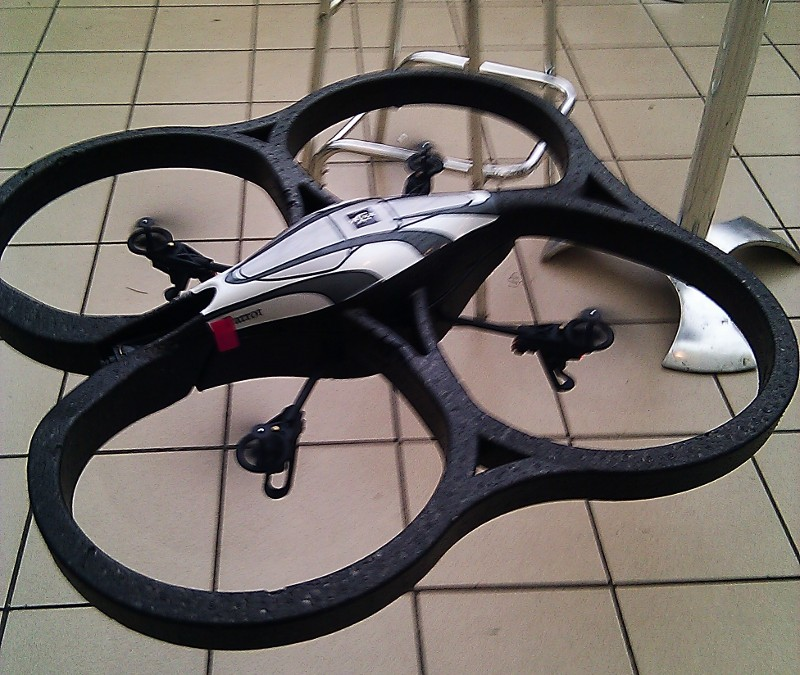
\includegraphics[width=0.5\textwidth]{img/ARDRONE}
  \end{figure}
  \begin{itemize}
    \item Two camera's (Front, Bottom)
    \item Sensors: accelerometers, gyroscopes, bottom-sonar
    \item Wifi
    \item OS: Linux
  \end{itemize}
\end{frame}

\subsection{Simulation}

\begin{frame}
  \frametitle{Tool: simulation}
  \begin{figure}
    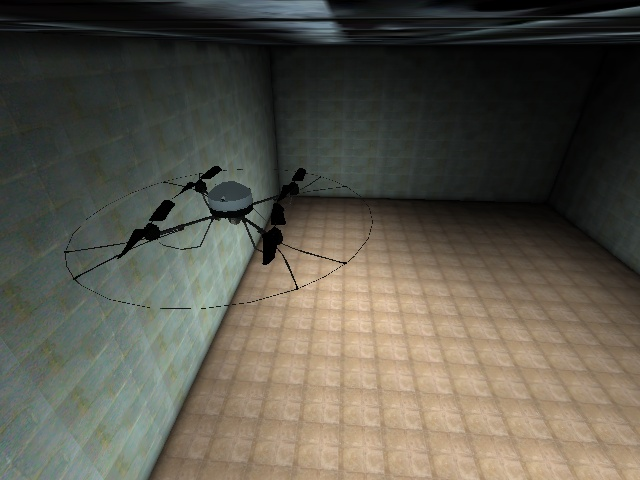
\includegraphics[width=0.5\textwidth]{img/AIRROBOT}
  \end{figure}
  \begin{itemize}
    \item Unreal tournament
    \item Airrobot edited
    \item Create simple levels
  \end{itemize}
\end{frame}

\section{Summary}

\begin{frame}
  \frametitle{Summary}
  \begin{itemize}
    \item How to find the optimal flying path (for general problems) using Reinforcement Learning?
    \item Practical test: what is the optimal path for a figure-8 flight?
  \end{itemize}
\end{frame}


\end{document}
